\documentclass{article}
\usepackage{graphicx} % Required for inserting images
\usepackage{amsmath} % helps formmating math
\usepackage{float} % helps formatting images
\title{Quarter Car Model with Single Mass}
\author{Justin Chin Cheong}
\date{May 2025}
\setlength{\parindent}{0pt} % kills the indent

\usepackage{listings}
\usepackage{xcolor}

\definecolor{mgreen}{rgb}{0,0.6,0}
\definecolor{mgray}{rgb}{0.5,0.5,0.5}
\definecolor{mblue}{rgb}{0,0,0.8}
\definecolor{mback}{rgb}{0.95,0.95,0.95}

\lstdefinestyle{matlabstyle}{
    language=Matlab,
    backgroundcolor=\color{mback},
    basicstyle=\ttfamily\footnotesize,
    keywordstyle=\color{mblue},
    commentstyle=\color{mgreen},
    stringstyle=\color{mgray},
    numberstyle=\tiny\color{mgray},
    numbers=left,
    numbersep=5pt,
    frame=single,
    breaklines=true,
    captionpos=b
}

\lstset{style=matlabstyle}


\begin{document}

\maketitle

\section{Problem Statement}
The quarter car model is a well known and widely applied model used to investigate the vertical dynamics of a vehicle. 

\vspace{1em}

It simplifies the the investigation to just a single tire with suspension. The version discussed here is the most simple case where there is some excitation from the road and only the mass of the car body is considered. The most important parameter is the acceleration of the body as it influences the comfort characteristics of the vehicle.

\vspace{1em}

Hence, the goal of this investigation is to:
\begin{enumerate}
    \item Characterize the system using basic system types
    %\item Investigate the step response of the system 
    \item Explore the frequency domain characteristics
\end{enumerate}

\subsection{Parameters}
To evaluate our model, we can use the following parameter values. 
\begin{align*}
    m &= 400kg\\
    c &= 20 000 \frac{N}{m} \\
    d &= 1500 \frac{Ns}{m} \\
\end{align*}

\section{Formulation}

\subsection{Ordinary Differential Equation}

\begin{figure}[H]
    \centering
    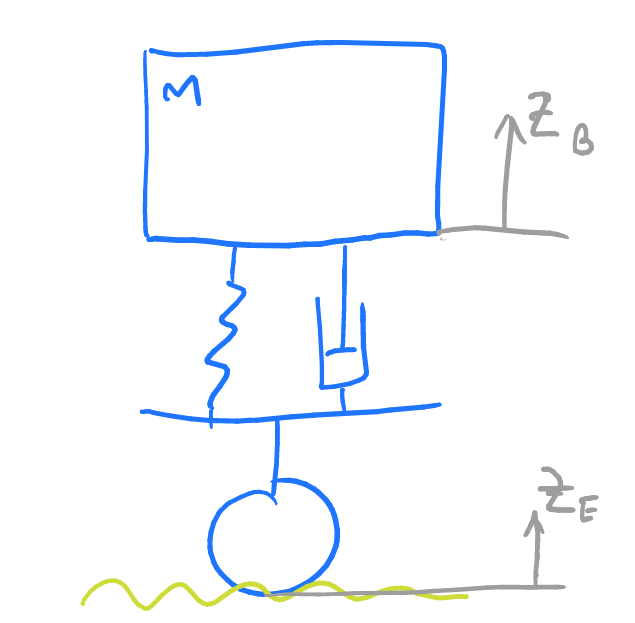
\includegraphics[width=0.5\linewidth]{systemdiagram.png}
    \caption{System diagram of quarter car model}
    \label{fig:SysD}
\end{figure}
To begin, we must of course do a freebody diagram.  

\begin{figure}[H]
    \centering
    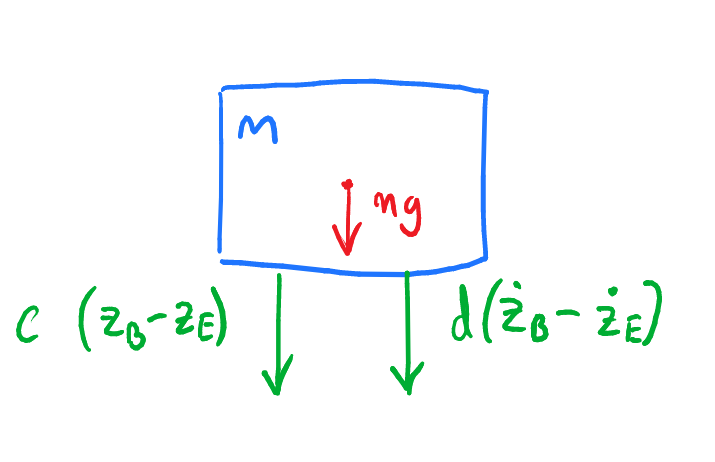
\includegraphics[width=0.5\linewidth]{freebodydiagram.png}
    \caption{Free body diagram of quarter car model}
    \label{fig:FBD}
\end{figure}

From fig.\ref{fig:FBD}, we get the following equilibrium. 

\begin{align}
\sum F=m\cdot\ddot{z}_{B} &=-mg-c(z_{B}-z_{E})-d(\dot{z}_{B}-\dot{z}_{E})
\label{eq:ODE}
\\
\ddot{z}_{B} &=-g-\frac{c}{m}z_{B}-\frac{d}{m}\dot{z}_{B}+\frac{c}{m}z_{E}+\frac{d}{m}\dot{z}_{E}
\label{eq:ODEexp}
\end{align}

This is our ordinary differential equation (ODE).

\subsection{Transfer Function}
We can performa a Laplace transform on \eqref{eq:ODEexp} considering $\ddot{z}_{B}$ as the output and $z_E$ as the input. We also assume the initial conditions are zero and body starts from a neutral position such that the static term $mg$ is of no consequence. (Alternatively we could have also excluded it from our free body diagram) 

\begin{align*}
    \mathscr{L}\{\ddot{z}_{B}(t) &=-\frac{c}{m}z_{B}(t)-\frac{d}{m}\dot{z}_{B}(t)+\frac{c}{m}z_{E}(t)+\frac{d}{m}\dot{z}_{E}(t)\}
    \\
    \Rightarrow\ddot{Z}_{B}(s) &= -\frac{c}{ms^2}\ddot{Z}_{B}(s)-\frac{d}{ms}\ddot{Z}_{B}(s)+\frac{c}{m}Z_{E}(s)+\frac{ds}{m}Z_{E}(s)
    \\
    \Leftrightarrow\ddot{Z}_{B}(s)\cdot(ms^2+ds+c) &= Z_E(s)\cdot(ds^3+cs^2)
    \\
    \Leftrightarrow \ddot{Z}_{B}(s) &= Z_E(s)\cdot \frac{s^2(ds+c)}{ms^2+ds+c}
\end{align*}
\\
Hence, we get a transfer function of 
\begin{equation}
    G_B(s)= \frac{s^2(ds+c)}{ms^2+ds+c}
    \label{eq:TF}
\end{equation}

\section{Analysis}
\subsection{System Characterization}
Using our transfer function \eqref{eq:TF}, we can find the poles and zeros to characterise it. 
\\
For the zeros:
\begin{align*}
    z_{1,2} &=0 \\
    z_3 &= -\frac{c}{d} \approx 13.333
\end{align*}
For the poles:
\begin{align*}
    p_{1,2} &=\frac{-d\pm\sqrt{d^{2}-4mc}}{2m}\\
    \Rightarrow p_1 &= \frac{-15+5\sqrt{119}\mathbf{i}}{8}\\
    \Rightarrow p_2 &= \frac{-15-5\sqrt{119}\mathbf{i}}{8}
\end{align*}
Having a zero at the the origin tells us that the system is differential while $z_3$ suggest proportionality. The presence of two poles also implies 2nd order delay. 

\vspace{1em}

As such we can characterise the system as a PDT2 system. 

\vspace{1em}

Additionally, we see that the real parts of both poles are less than zero and hence the system is stable. It can also be noted that the system is not causal, but for our purposes, that is fine. 

% \subsection{Step Response}
% To find the step response, we must first consider that the poles can be expressed in the form $$p_{1,2}=\alpha\pm\beta\mathbf{i}$$

% Such that the transfer function can be standardised as

% \begin{equation*}
%     G_B(s)=\frac{1}{d}\frac{s^2(s+\frac{c}{d})}{(s-(\alpha+\beta \mathbf{i}))(s-(\alpha-\beta \mathbf{i}))}
% \end{equation*}

% Which simplifies to 

% \begin{equation}
%     G_B(s)=\frac{1}{d}\frac{s^2(s+\frac{c}{d})}{(s-\alpha)^2+\beta^2}
% \end{equation}

\subsection{Frequency Domain Characteristics}
Using our transfer function, we can plot a bode diagram to illustrate the frequency domain characterstics.

\vspace{1em}

We can actually do this quite easily using MATLAB. 
\begin{lstlisting}[language=Matlab, caption={Script to Plot Bode Diagrams}]
%% Programm

close all
clear all
m = 400;  % mass
c = 20000; % stiffness
d = 1500; % damping
F = 1000; % external load
g = 981/100; % gravity
z0 = m*g/c; % initial displacement
freq={0,50*(2*pi)};

%% Bode Plot
sys = tf([d,c,0,0],[m,d,c]);

bode(sys,freq)
xlabel('Frequency [rad/s]')
title('Bode Plot of Body Acceleration Transfer Function due to Road Excitation')
\end{lstlisting}

This code gives us the following plot

\begin{figure} [H]
    \centering
    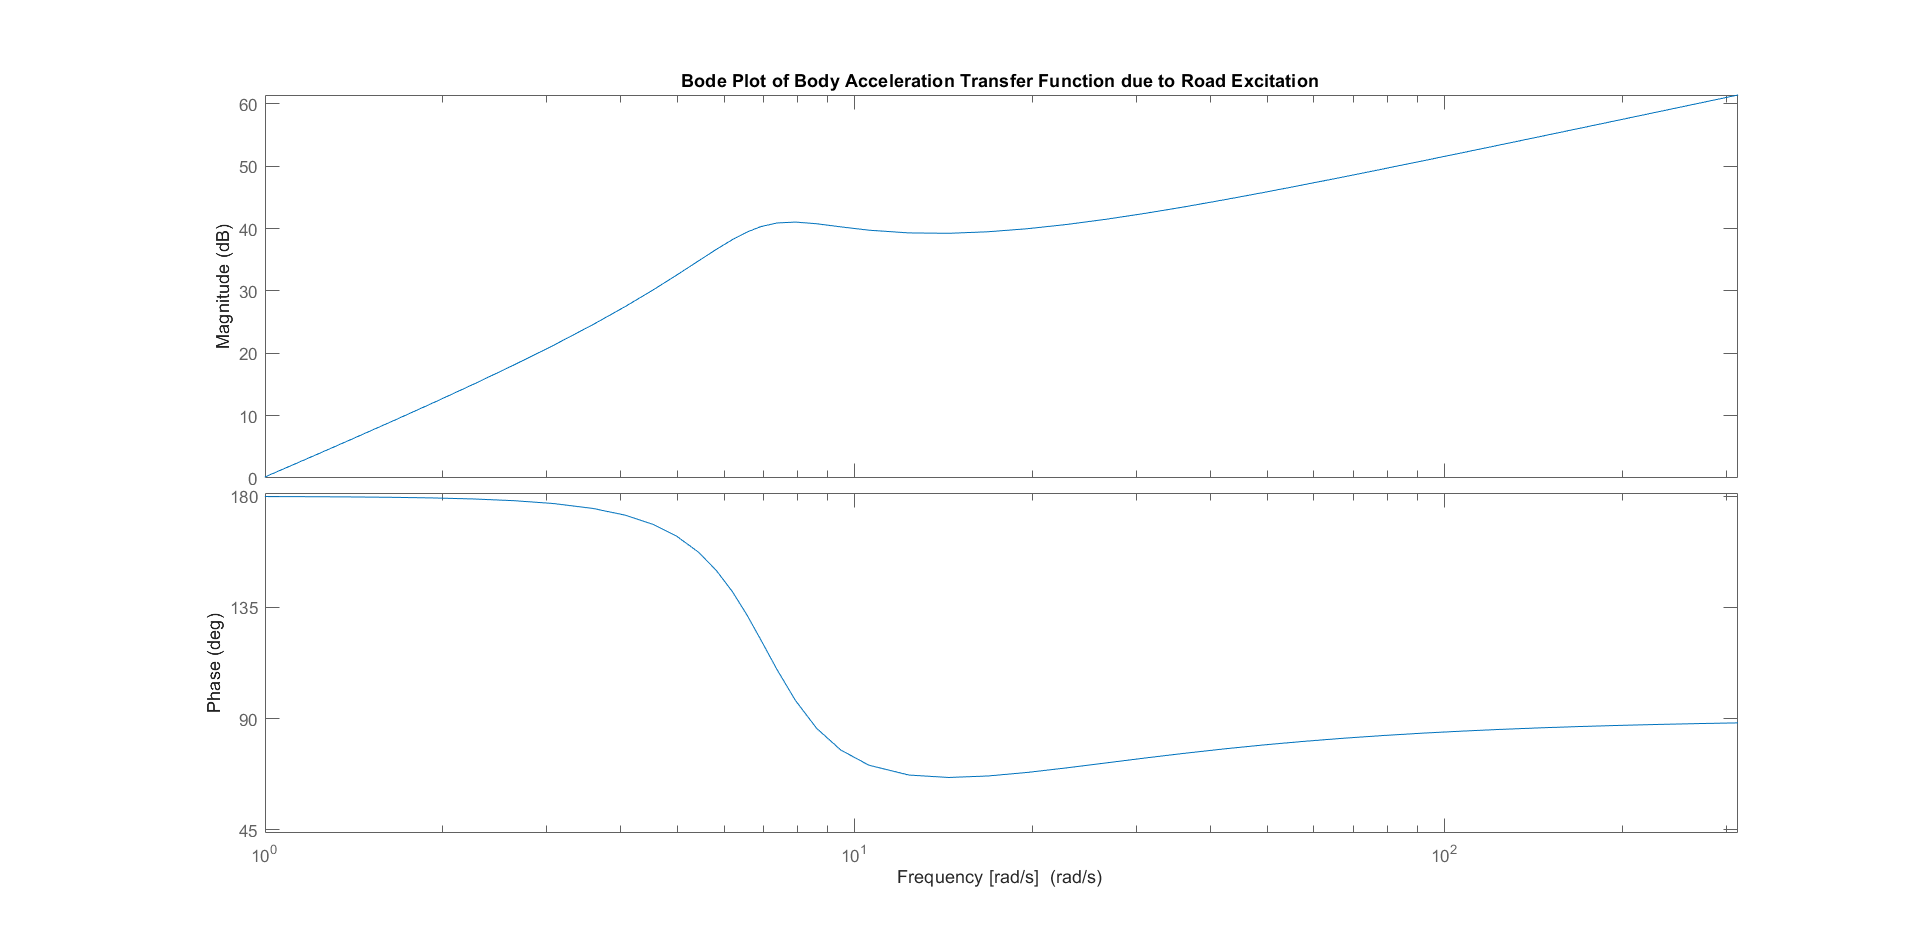
\includegraphics[width=1\linewidth]{BodePlot_SingleMass_Acc.png}
    \caption{Bode Plot of $G_B(s)$}
    \label{fig:BodePlot}
\end{figure}

\vspace{1em}

With MATLAB, we can even go a bit further and investigate how different parameters change the bode plot. 

\begin{lstlisting}[language=Matlab, caption={Script to Plot Bode Diagram Varying Mass}]
%% Variation of Mass
% Initialisation of parameters done in previous listing
mass=100:100:1000;

for h=1:length(mass)
    m = mass(h);  % update the mass
    leg(h)= mass(h) + " kg"; % storing mass for legend
    sys_acc(h)=tf([d,c,0,0],[m,d,c]); % finding transfer function
end

bode(sys_acc(1),sys_acc(2),sys_acc(3),sys_acc(4),sys_acc(5),sys_acc(6),sys_acc(7),sys_acc(8),sys_acc(9),sys_acc(10),freq)
acc_leg = legend(leg);
acc_leg.Location = 'southeast';
title('Bode Plot of Body Acceleration as body mass varies')
\end{lstlisting}

\begin{figure} [H]
    \centering
    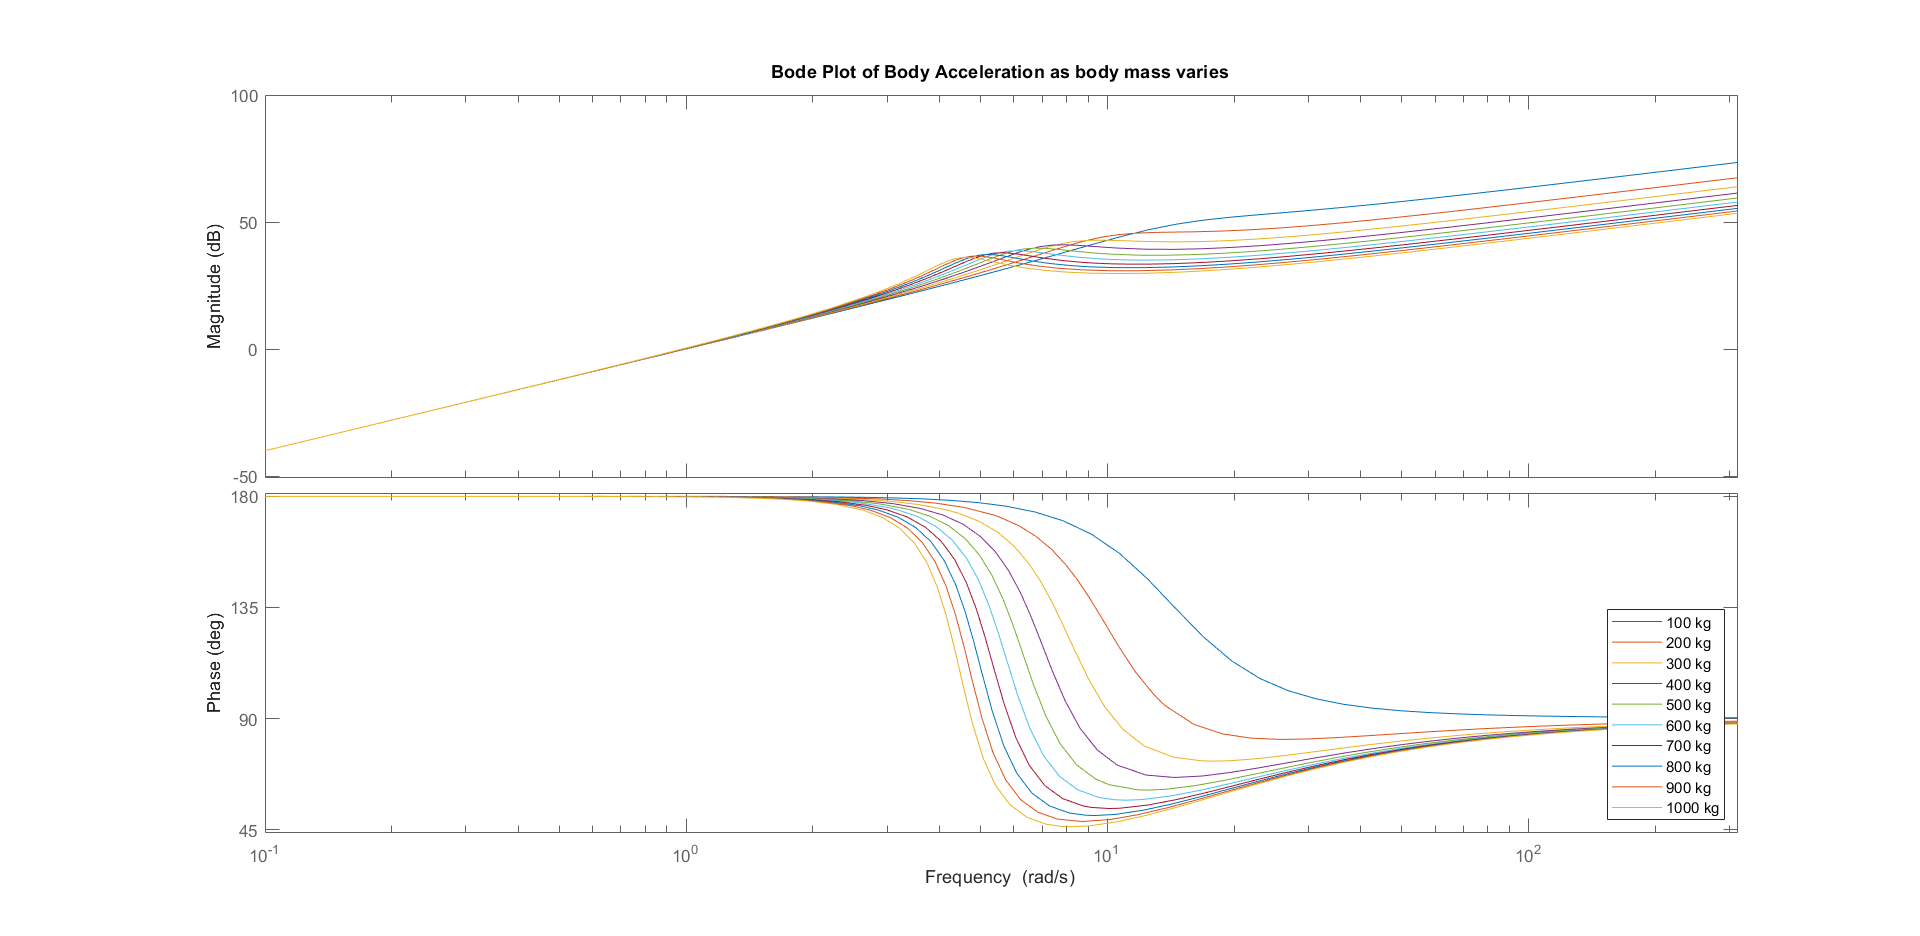
\includegraphics[width=1\linewidth]{BodePlot_SingleMass_Acc_MassVar.png}
    \caption{Bode Plot of $G_B(s)$ while varying mass $m$}
    \label{fig:BodePlotMassVar}
\end{figure}

To accomplish the same plots manually, we must consider the transfer function as $$s\rightarrow \omega\mathbf{i}$$

\begin{equation}
    G(jw)=\frac{-d\omega^{3}\mathbf{i}-c\omega^{2}}{-m\omega^{2}+d\omega \mathbf{i}+c}
\end{equation}

For the magnitude: 
\begin{align*}
A(w) &:=|G(w\mathbf{i})| \\
 &=\left|\frac{-d\omega^{3}\mathbf{i}-c\omega^{2}}{-m\omega^{2}+d\omega \mathbf{i}+c}\right| \\
 &=\frac{\sqrt{(c\omega^2)^{2}+(d\omega^{3})^{2}}}{\sqrt{(c-m\omega^{2})^{2}+(d\omega)^{2}}} \\
A(w) &=\sqrt{\frac{(c\omega^{2})^{2}+(d\omega^{3})^{2}}{(c-m\omega^{2})^{2}+(d\omega)^{2}}}
\end{align*}

For the phase: 
\begin{align*}
    \phi(\omega) &:=\angle G_{B}(\omega \mathbf{i}) \\
 &=\arg\left(\frac{-d\omega^3\mathbf{i}-c\omega^2}{-m\omega^2+d\omega \mathbf{i}+c}\right) \\
 &=\arg(-d\omega^3\mathbf{i}-c\omega^2)-\arg(-m\omega^2+d\omega \mathbf{i}+c) \\
\phi(\omega) &=\arctan\left(\frac{d\omega}{c}\right)-\arctan\left(\frac{d\omega}{c-m\omega^2}\right)
\end{align*}

Now, in MATLAB. 

\begin{lstlisting}[language=Matlab, caption={Script to Plot Bode Diagram Manually}]
%% Manual Bode
A = @(w)(sqrt(((c*w^2)^2+(d*w^3)^2)/((c-m*w^2)^2+(d*w)^2)));
% Using angle since arctan doesn't work well
phi = @(w)(angle((-c*w^2-d*(w^3)*1i)/(c-m*w^2+d*w*1i))); 

w = linspace(1,50*2*pi,1000);

for k=1:length(w)
A_val(k) = feval(A,w(k)); phi_val(k) = phi(w(k));
end

subplot(2,1,1)
loglog(w,A_val)
xlabel('Frequency [rad/s]')
ylabel('Amplitude')
title('Bodeplot') 

subplot(2,1,2)
loglog(w,phi_val)
xlabel('Frequency [rad/s]')
ylabel('Phase')
\end{lstlisting}

\begin{figure} [H]
    \centering
    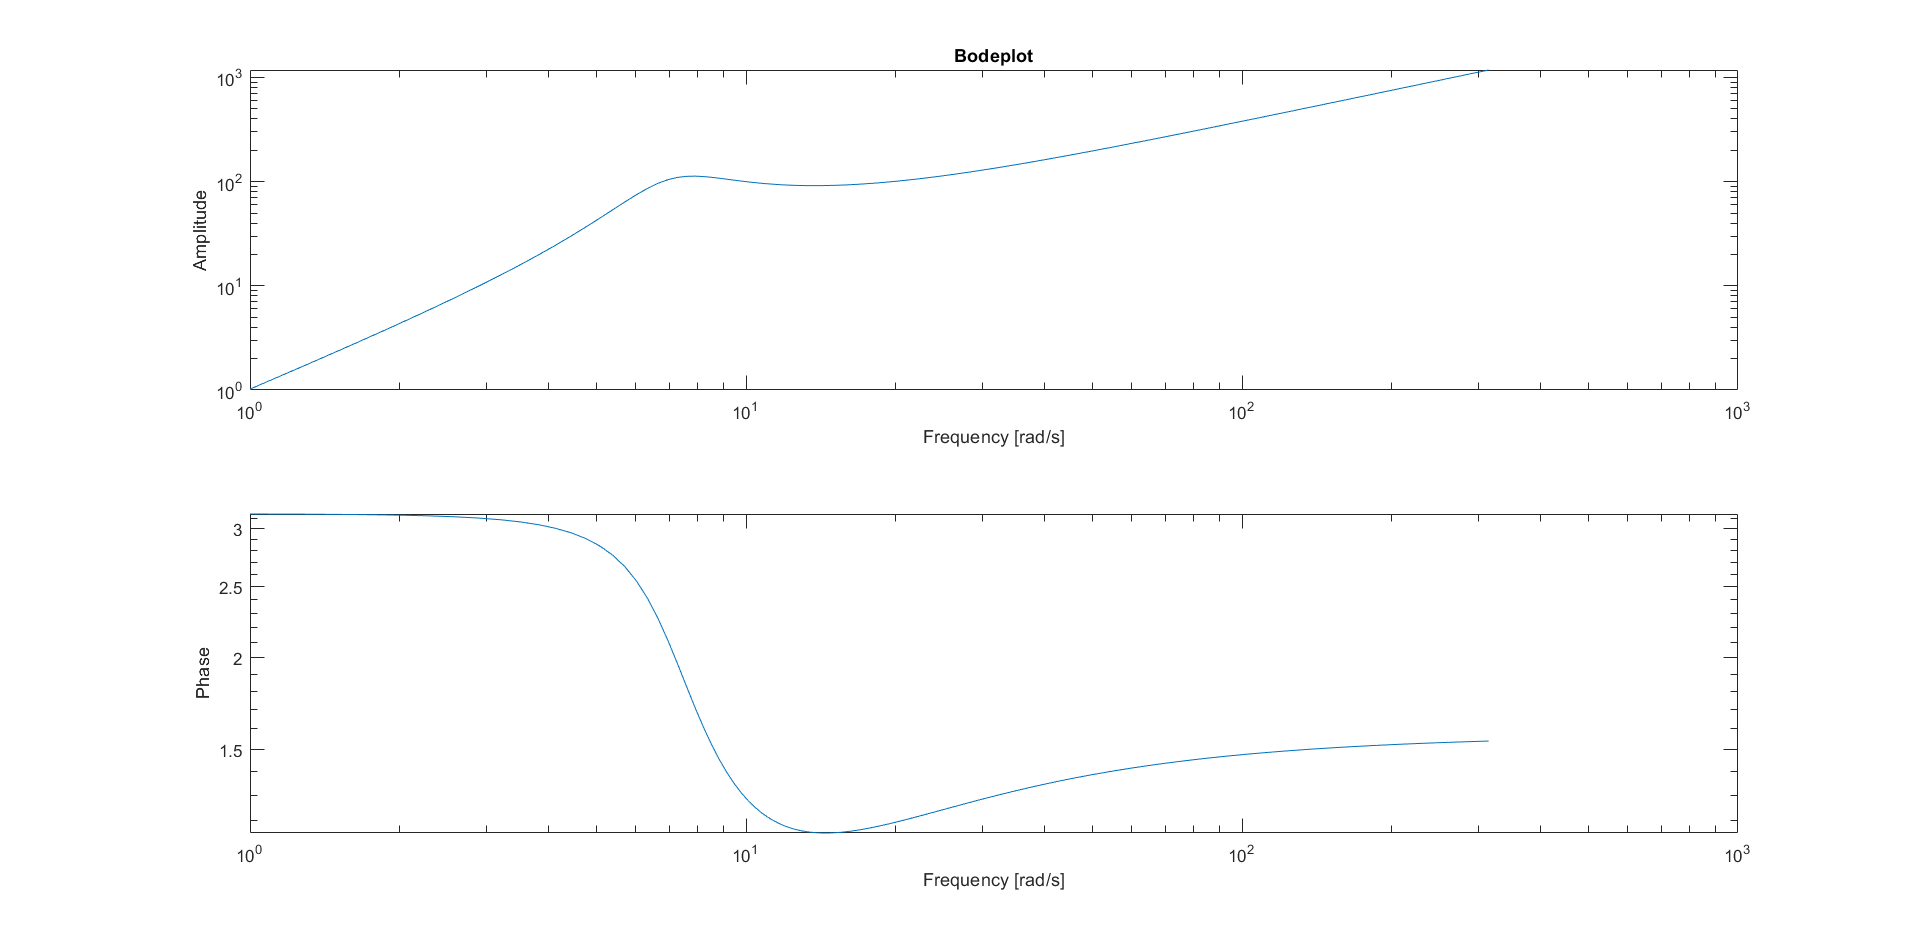
\includegraphics[width=1\linewidth]{BodePlot_SingleMass_Acc_Manual.png}
    \caption{Bode Plot of $G_B(s)$ using manual method}
    \label{fig:BodePlotManual}
\end{figure}

\end{document}
